\begin{frame}{Precision estimates at the LHC}
  \framesubtitle{Evidence for Beyond-Standard-Model physics}

  \begin{columns}

    \begin{column}{0.5\textwidth}

      \begin{figure}
        \centering
        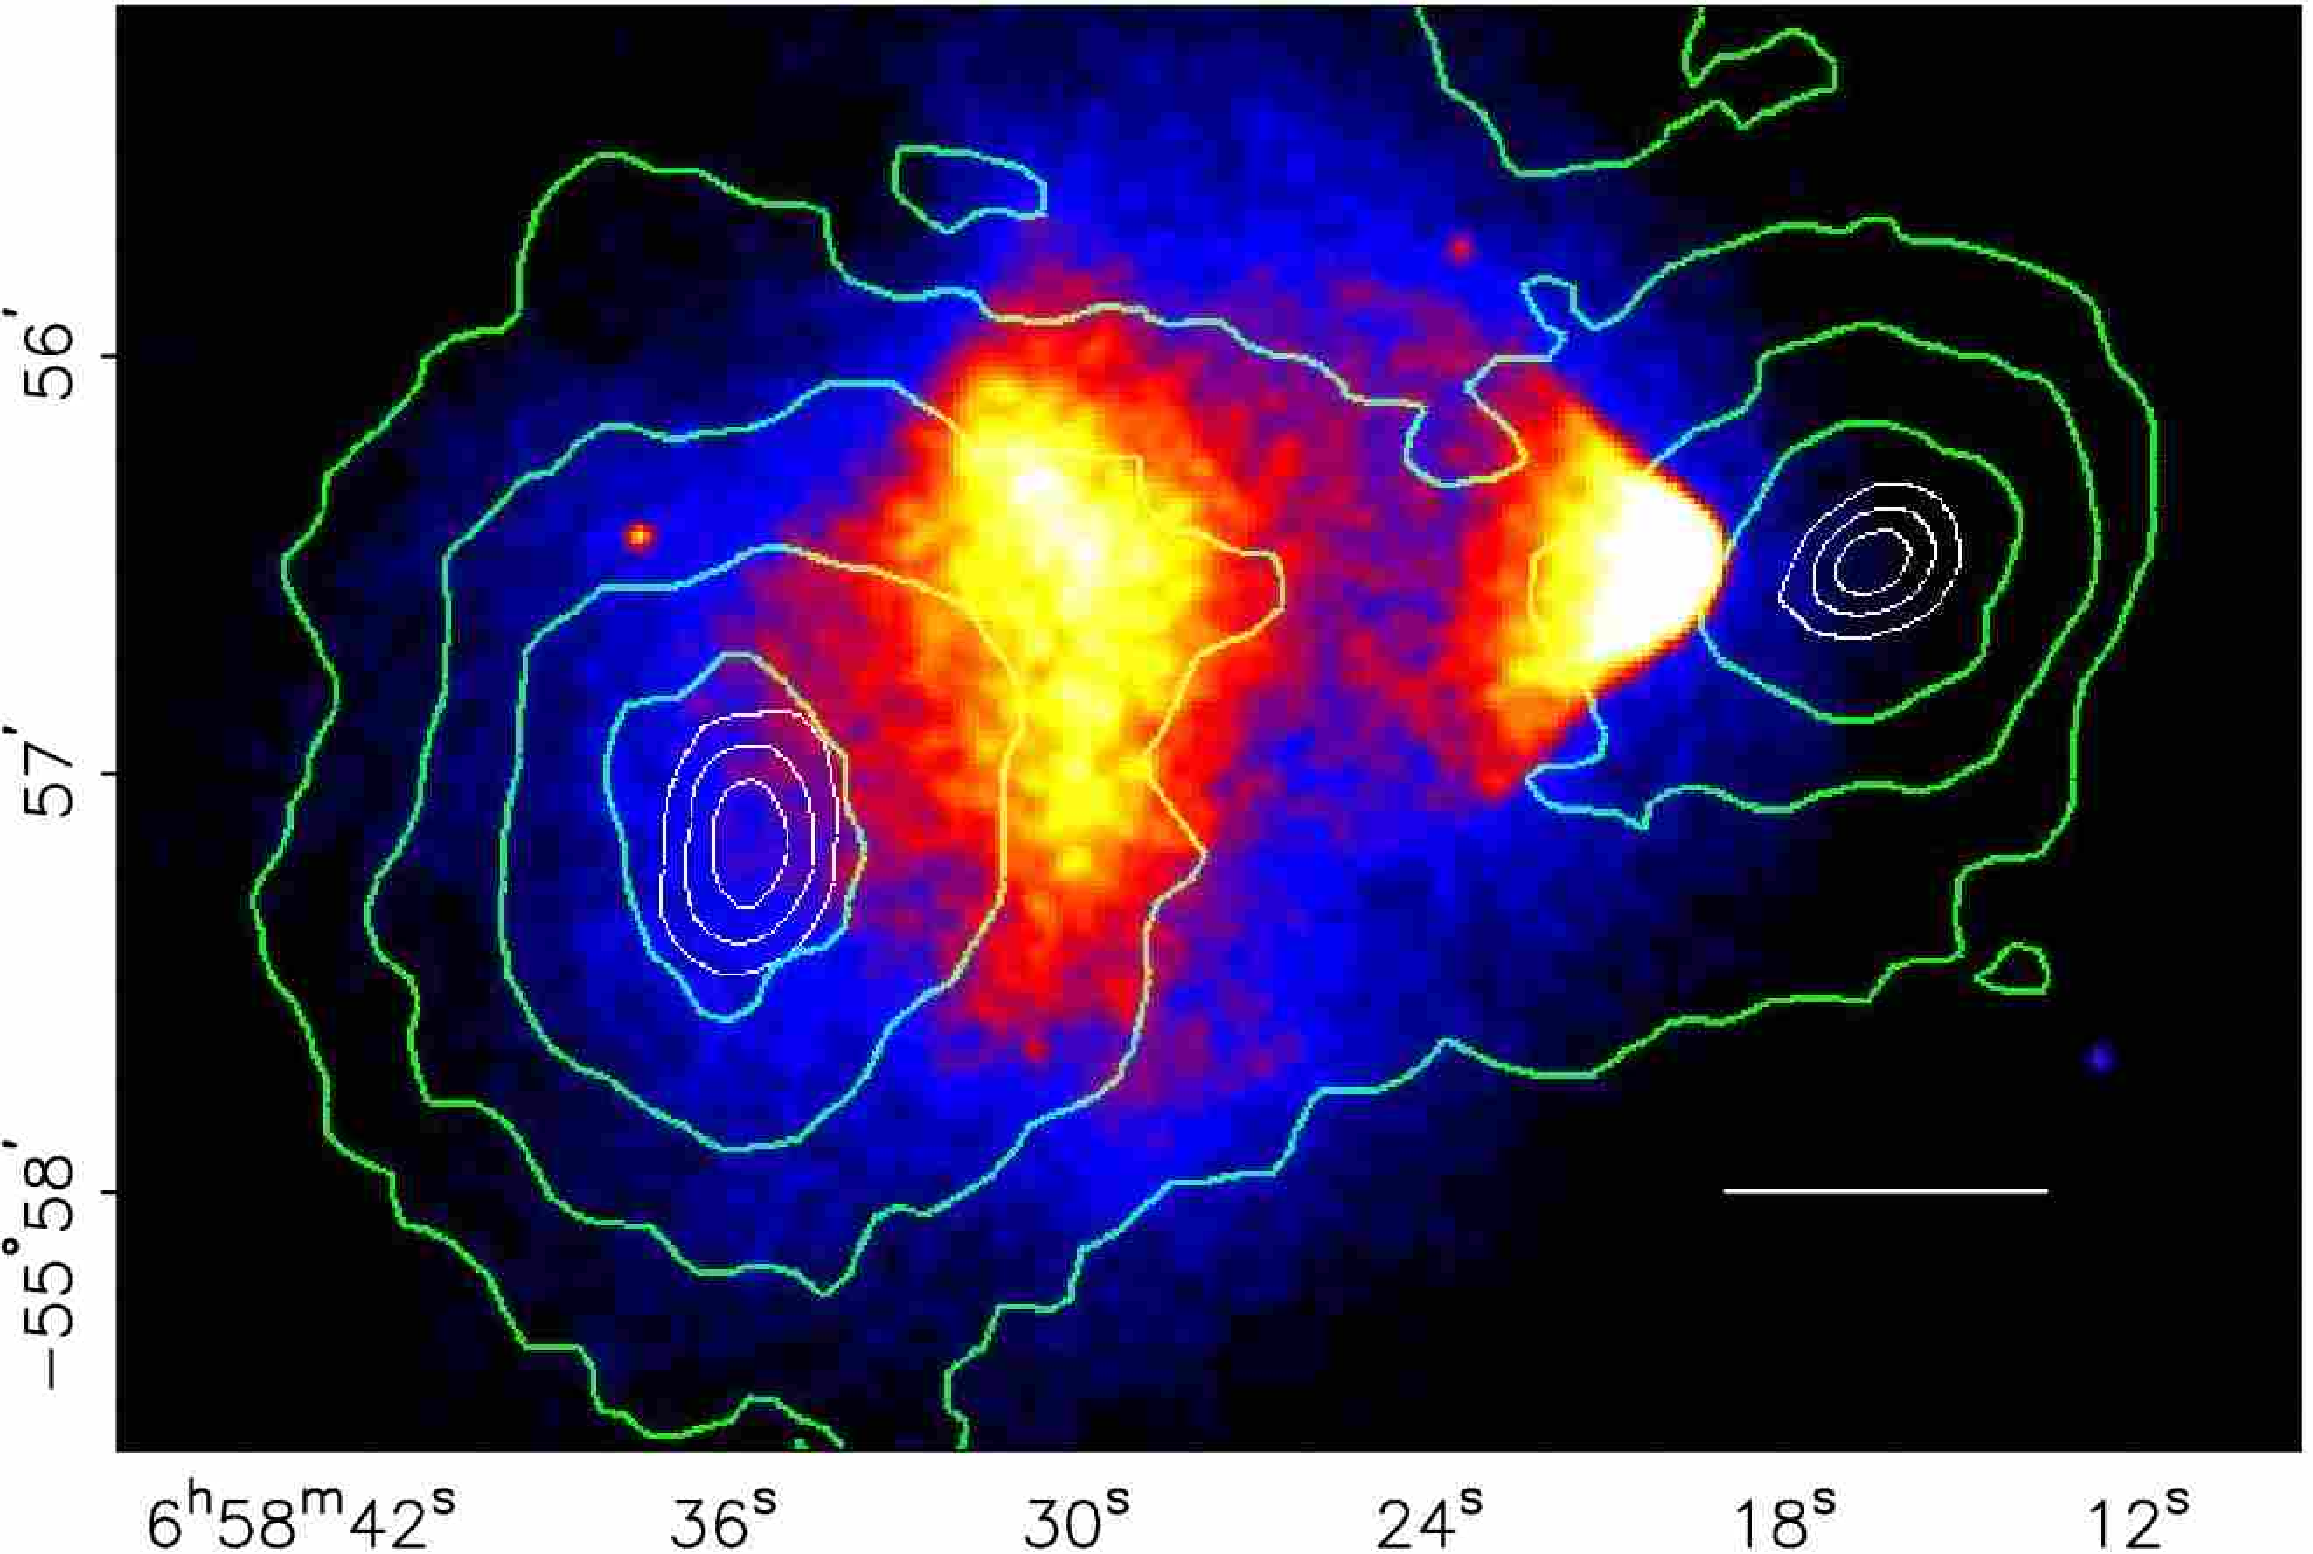
\includegraphics[width = \textwidth]{imgs/clowe-2.png}
      \end{figure}

    \end{column}

    \begin{column}{0.5 \textwidth}

      \begin{colorblock}[black]{statalegrey}{Main BSM evidence}
        \begin{itemize}
          \item dark matter and dark energy
          \item matter-antimatter asymmetry
          \item neutrino masses
        \end{itemize}
      \end{colorblock}

      \vspace{0.5em}


      \capcol{Figure} from Clowe et al. 2006.

      \justifying
      Offset between the observed baryonic mass distribution and the gravitational potential in the Bullet Cluster (1E 0657-56).

    \end{column}

  \end{columns}

\end{frame}

%=======================================================================

\begin{frame}{Precision estimates at the LHC}
  \framesubtitle{BSM constraints and shift in research paradigm}

  \begin{columns}

    \begin{column}{0.5 \textwidth}

      \begin{colorblock}[black]{statalegrey}{Main BSM proposals}
        \begin{itemize}
          \item supersymmetric models (MSSM, \dots)
          \item dark matter models (WIMPs, axions, \dots)
          \item extended gauge sectors ($ \mathrm{SO}(10) $, \dots)
          \item SM Effective Field Theory (SMEFT)
        \end{itemize}
      \end{colorblock}

      \vspace{0.5em}

      \capcol{Figure} from ATLA PUB Note 2023--025.

      \justifying
      Exclusion limits in the $ \tilde{g} - \tilde{\chi}^0_1 $ mass plane for various models for the decay of the gluino to the lightest supersymmetric particle.

    \end{column}

    \begin{column}{0.5\textwidth}

      \begin{figure}
        \centering
        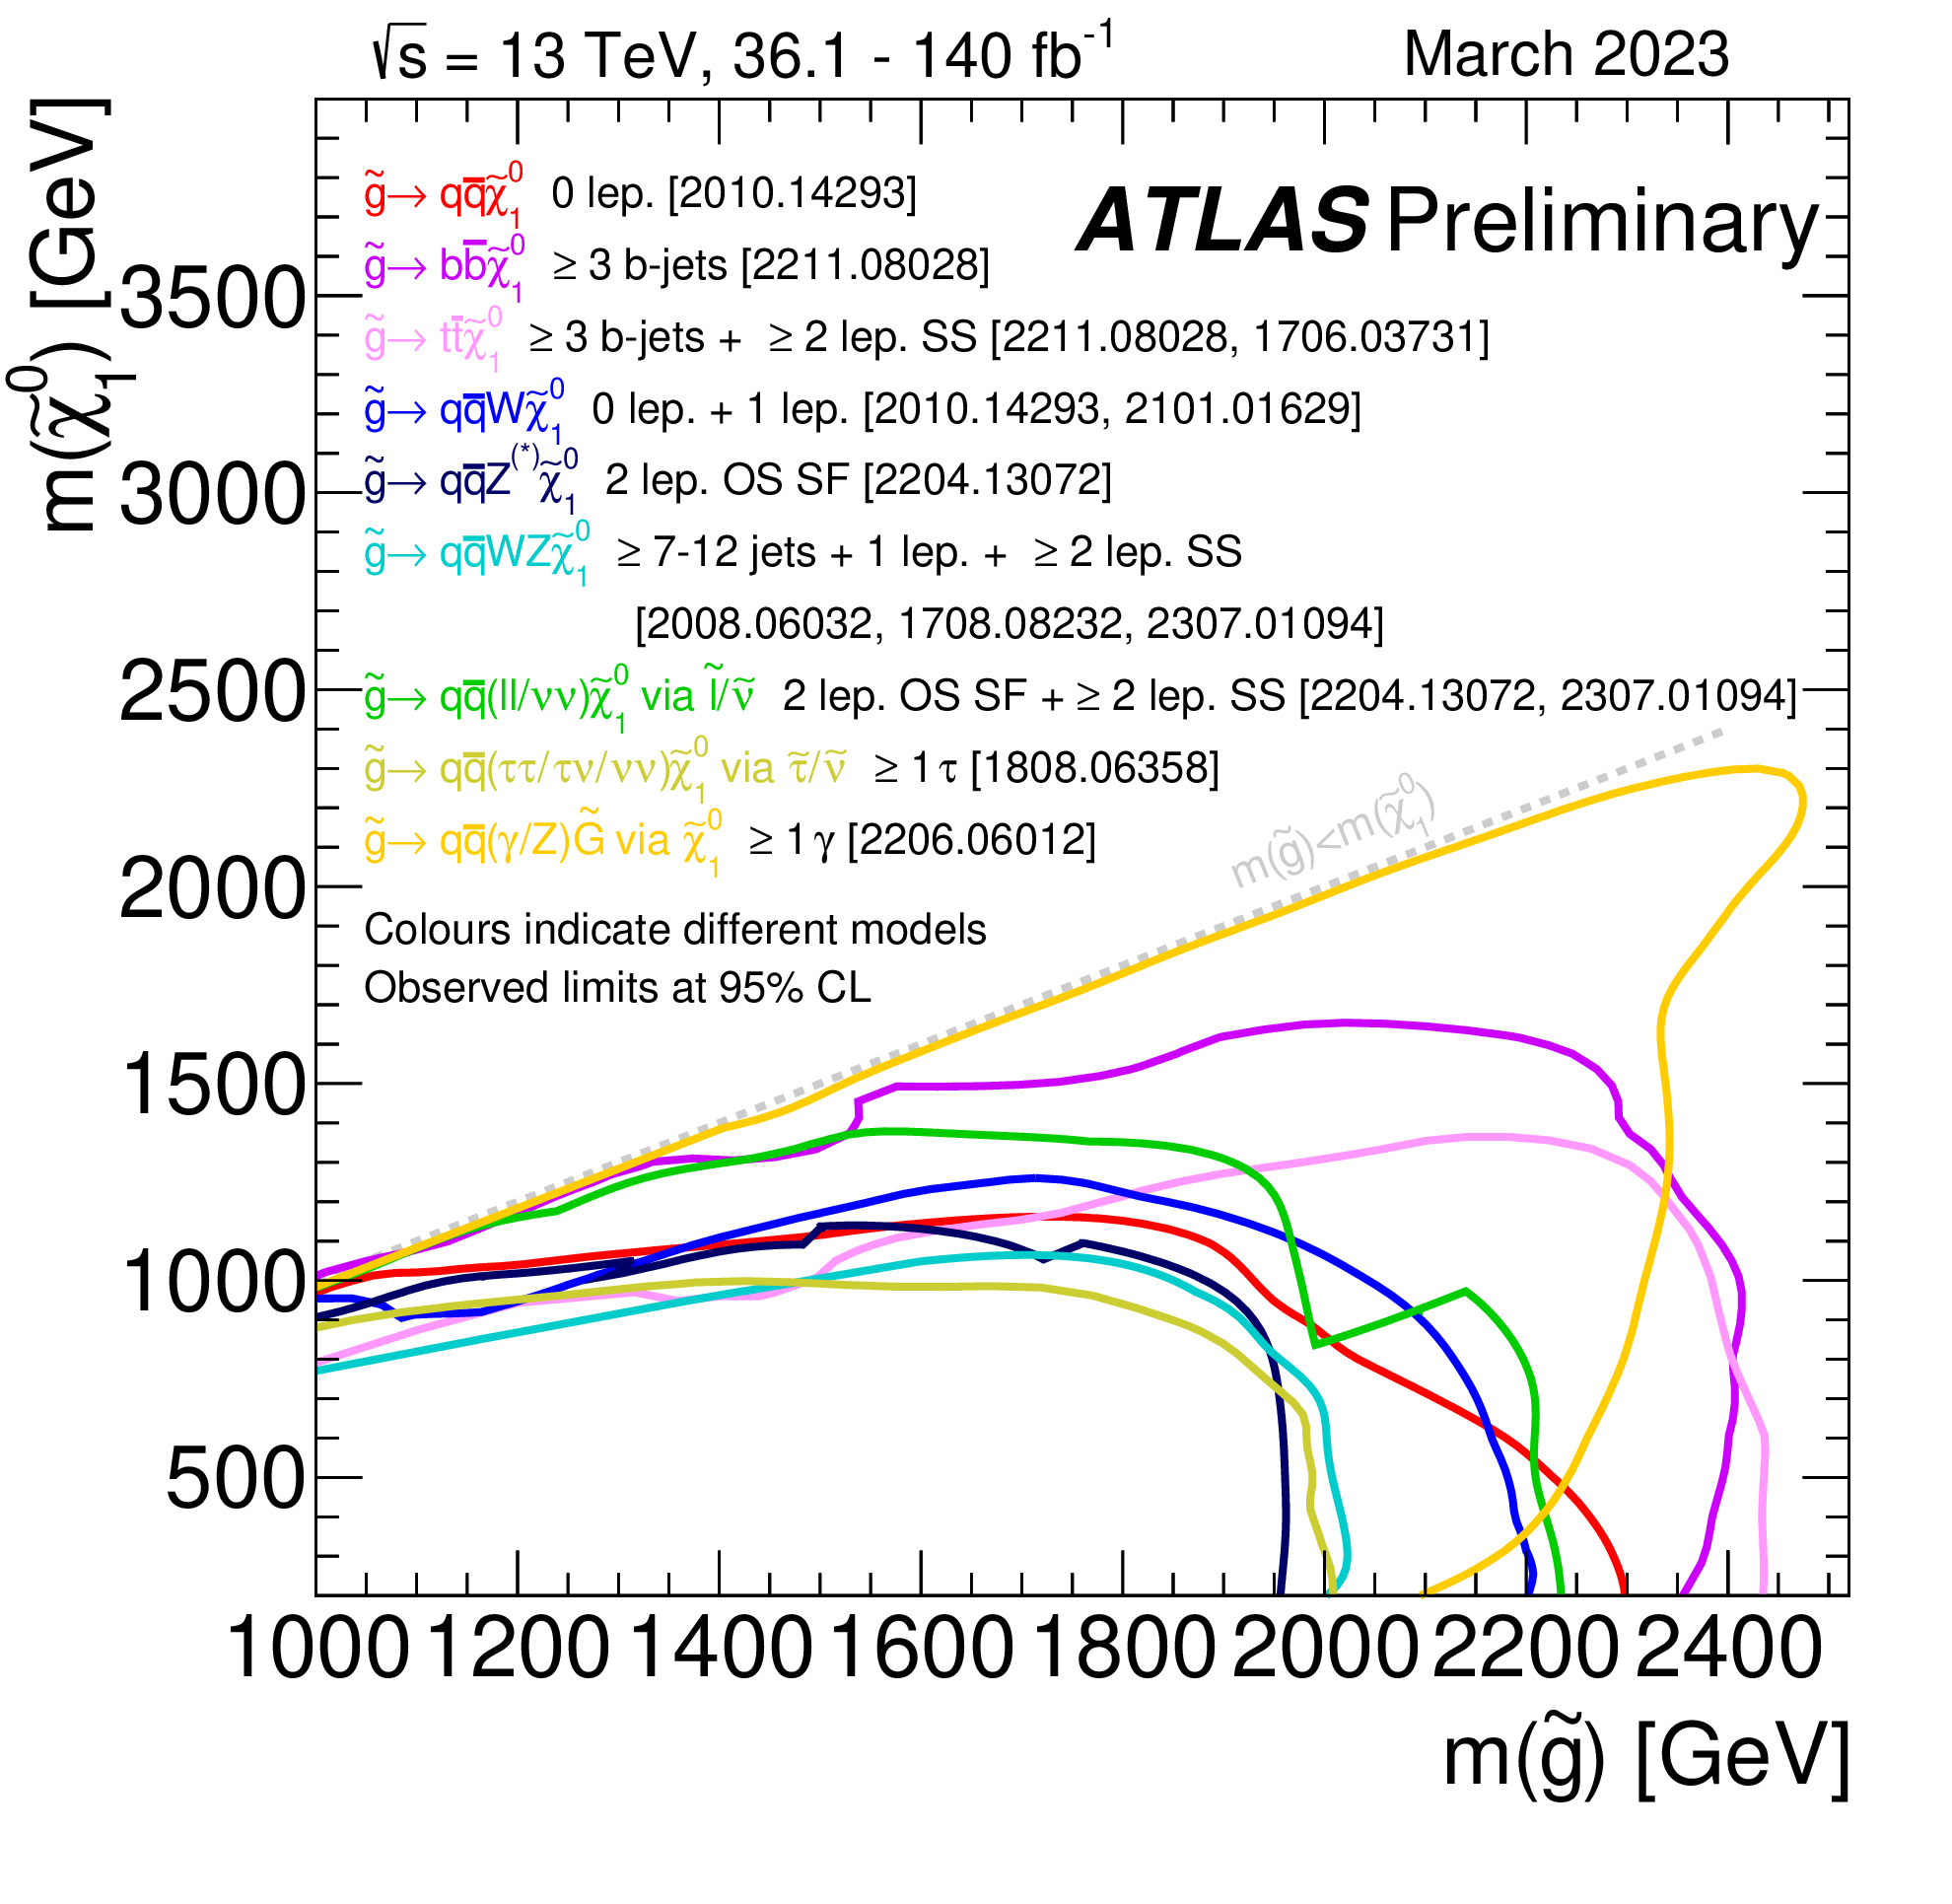
\includegraphics[width = 0.94\textwidth]{imgs/susy.png}
      \end{figure}

    \end{column}

  \end{columns}

\end{frame}

%=======================================================================

\begin{frame}{Precision estimates at the LHC}
  \framesubtitle{Factorization theorem and perturbative QCD}

  factorization theorem and perturbative expansion of $ \mathrm{d} \hat{\sigma}_{a,b} $

\end{frame}

%=======================================================================

\begin{frame}{IR-pole structure of QCD}
  \framesubtitle{Radiative correction to partonic processes}

  real and virtual corrections

\end{frame}

%=======================================================================

\begin{frame}{IR-pole structure of QCD}
  \framesubtitle{Dimensional Regularization of IR singularities}

  soft and collinear singularities (in CDR, show in real corrections)

\end{frame}

%=======================================================================

\begin{frame}{IR-pole structure of QCD}
  \framesubtitle{Subtraction schemes}

  subtraction scheme to regulate divergences

\end{frame}

%=======================================================================

\begin{frame}{NSC subtraction scheme}
  \framesubtitle{Extraction of poles via operators}

  introduce the NSC SS

\end{frame}

%=======================================================================

\begin{frame}{NSC subtraction scheme}
  \framesubtitle{Pole cancellation}

  briefly show pole cancellation in the NSC SS

\end{frame}

%=======================================================================

\begin{frame}{NSC SS with massive quarks}
  \framesubtitle{Mass-regualtion of soft and collinear limits}

  explain why massive quarks change $ I_\text{S}(\epsilon) $ and $ I_\text{V}(\epsilon) $, but not $ I_\text{C}(\epsilon) $

\end{frame}

%=======================================================================

\begin{frame}{NSC SS with massive quarks}
  \framesubtitle{Generalized soft operator}

  show how $ I_\text{S}(\epsilon) $ changes (in particular massive angular integrals)

\end{frame}

%=======================================================================

\begin{frame}{NSC SS with massive quarks}
  \framesubtitle{Generalized virtual operator}

  show how $ I_\text{V}(\epsilon) $ changes (in particular, colour-correlated $ \epsilon^{-2} $-poles in $ \mathcal{V}_{i,j}(\epsilon) $ coefficients)

\end{frame}

%=======================================================================

\begin{frame}{NSC SS with massive quarks}
  \framesubtitle{Pole cancellation: generalized pole terms}

  highlights of pole cancellation in $ I_{\text{S}+\text{V}}(\epsilon) $, define $ \chi_{i,j}(\epsilon) $ coefficients and explain their property

\end{frame}

%=======================================================================

\begin{frame}{NSC SS with massive quarks}
  \framesubtitle{Pole cancellation: colour-correlated terms}

  show pole cancellation in the colour-correlated sum of $ I_{\text{S}+\text{V}}(\epsilon) $, leaving the same (and opposite) pole terms of $ I_\text{C}(\epsilon) $

\end{frame}

%=======================================================================

\begin{frame}{NSC SS with massive quarks}
  \framesubtitle{Generalized integrated counterterms}

  show integrated counterterms and highlighting massive logs

\end{frame}


%=======================================================================

\begin{frame}{Conclusions}
  \framesubtitle{Future developments}

  draw conclusions and point out possible further developments

\end{frame}










